% ╔══════════════════════════════════════════════════════════════════════════════╗
% ║  Harry Bevins – Beamer Presentation Template                               ║
% ║  Style based on 2025/2026 Keynote talks (white, clean, sans-serif)         ║
% ╚══════════════════════════════════════════════════════════════════════════════╝
%
% Quick-start: edit the \talkinfo block below, then add frames.
%
% Compile with:  pdflatex bevins-beamer.tex
% or:            lualatex bevins-beamer.tex   (recommended for better fonts)

\documentclass[aspectratio=169, 12pt]{beamer}

% ─── Fonts ────────────────────────────────────────────────────────────────────
% Option A (pdflatex): Helvetica clone
\usepackage[T1]{fontenc}
\usepackage{helvet}
\renewcommand{\familydefault}{\sfdefault}

% Option B (lualatex/xelatex): Closer match to Keynote's feel – uncomment to use
% \usepackage{fontspec}
% \setsansfont{Helvetica Neue}   % macOS; or try "TeX Gyre Heros" (free)
% \setmainfont{Helvetica Neue}

\usepackage{microtype}

% ─── Math ─────────────────────────────────────────────────────────────────────
\usepackage{amsmath, amssymb}

% ─── Graphics & Layout ────────────────────────────────────────────────────────
\usepackage{graphicx}
\usepackage{booktabs}

% ─── Hyperlinks ───────────────────────────────────────────────────────────────
\usepackage{hyperref}
\hypersetup{
    colorlinks = true,
    urlcolor   = blue,
    linkcolor  = black,
    citecolor  = black,
}

% ─── Colors ───────────────────────────────────────────────────────────────────
\usepackage{xcolor}
\definecolor{footergray}{RGB}{130, 130, 130}
% Accent colour: used sparingly (e.g. highlighted text, overlays).
% Matches the dark navy found in section-divider slides.
\definecolor{accentblue}{RGB}{20, 40, 100}

% ══════════════════════════════════════════════════════════════════════════════
%  TALK METADATA  –– edit this block for each new talk
% ══════════════════════════════════════════════════════════════════════════════
\newcommand{\talktitle}{Revealing the Cosmic Dark Ages from lunar orbit with CosmoCube}
\newcommand{\talkauthor}{Harry T.\ J.\ Bevins}
\newcommand{\talkposition}{Kavli Fellow}
\newcommand{\talkinstitute}{Kavli Institute for Cosmology, University of Cambridge}
\newcommand{\talkconfooter}{NAM 2026 University of Birmingham}   % appears in footer
\newcommand{\talkemail}{htjb2@cam.ac.uk}
% arXiv tag – leave empty {} to suppress
\newcommand{\talkarxiv}{}
% \newcommand{\talkarxiv}{arXiv:2503.13263}

% ══════════════════════════════════════════════════════════════════════════════
%  BEAMER APPEARANCE
% ══════════════════════════════════════════════════════════════════════════════

\setbeamertemplate{navigation symbols}{}        % no nav buttons

% Background & text
\setbeamercolor{background canvas}{bg=white}
\setbeamercolor{normal text}{fg=black, bg=white}

% Frame title: top-left, bold, plain black text – no box/bar
\setbeamercolor{frametitle}{fg=black, bg=white}
\setbeamerfont{frametitle}{size=\large, series=\bfseries}
\setbeamertemplate{frametitle}{%
    \vspace{0.45em}%
    \insertframetitle%
}

% Bullets: large filled circle, then dashes for sub-items
\setbeamercolor{item}{fg=black}
\setbeamercolor{subitem}{fg=black}
\setbeamercolor{subsubitem}{fg=black}
\setbeamertemplate{itemize item}{\large$\bullet$}
\setbeamertemplate{itemize subitem}{--}
\setbeamertemplate{itemize subsubitem}{$\circ$}
\setlength{\leftmargini}{1.2em}

% ─── Footer ───────────────────────────────────────────────────────────────────
% Layout: [bold gray "Conference, Date – email"] ........ [arXiv]  [page]
\setbeamertemplate{footline}{%
    \begin{beamercolorbox}[wd=\paperwidth, ht=2.4ex, dp=1.4ex]{footline}
        \hspace*{0.025\paperwidth}%
        {\color{footergray}\scriptsize\textbf{\talkconfooter{} -- \talkemail}}%
        \hfill
        \ifx\talkarxiv\empty\else
            {\color{blue}\scriptsize\talkarxiv}%
            \hspace{0.8em}%
        \fi
        {\color{footergray}\scriptsize\insertframenumber}%
        \hspace*{0.025\paperwidth}%
    \end{beamercolorbox}%
}

% ─── Title page ───────────────────────────────────────────────────────────────
\setbeamertemplate{title page}{%
    \vspace{0.10\paperheight}
    \begin{center}
        % Large bold title
        {\bfseries\LARGE\talktitle\par}
        \vspace{0.9em}
        % Author and position
        {\large\talkauthor\par}
        \vspace{0.25em}
        {\normalsize\talkposition\par}
        \vspace{1.4em}
        % Logos row – add/remove \includegraphics lines as needed
        %
        
\includegraphics[height=1.1cm]{../../../beamer-template/logos/cambridge.png}\hspace{0.6cm}%
        
\includegraphics[height=1.1cm]{../../../beamer-template/logos/kicc.png}\hspace{0.6cm}%
        
\includegraphics[height=1.1cm]{../../../beamer-template/logos/cavendish.png}\hspace{0.6cm}%
        
\includegraphics[height=1.1cm]{../../../beamer-template/logos/reach.png}\hspace{0.6cm}%
        
\includegraphics[height=1.1cm]{../../../beamer-template/logos/cosmocube.png}%
        %
    \end{center}
}

% ──  Helper: section-divider frame  ──────────────────────────────────────────
% Usage: \sectionframe{Section Title Text}
\newcommand{\sectionframe}[1]{%
    \begin{frame}{}
        \vfill
        \begin{center}
            {\large #1}
        \end{center}
        \vfill
    \end{frame}%
}

% ══════════════════════════════════════════════════════════════════════════════
\begin{document}
% ══════════════════════════════════════════════════════════════════════════════

% ── Title slide ───────────────────────────────────────────────────────────────
\begin{frame}{}
    \titlepage
\end{frame}

% ══════════════════════════════════════════════════════════════════════════════
%  SECTION 1
% ══════════════════════════════════════════════════════════════════════════════

\sectionframe{The Cosmic Dark Ages}

% Introduce the science of the dark ages... 
\begin{frame}{The Sky Averaged 21-cm Signal}
    \begin{columns}[T]
        \begin{column}{0.55\textwidth}
            \begin{itemize}
                \item Arises from the spin flip transition in neutral hydrogen
                \item Statistical temperature which quantifies the number of atoms in each state
                \item Measure this temperature relative to the CMB over cosmological time
                \item Transition driven by CMB photons, collisions between atoms and eventually astrophysics
                \item The dark ages is purely cosmology
            \end{itemize}
        \end{column}
        \hfill
        \begin{column}{0.4\textwidth}
            \centering
            \includegraphics[width=\textwidth]{example-image}  % replace with figure
            \\[0.3em]
            {\small Optional caption text}
        \end{column}
    \end{columns}
\end{frame}

% How does the signal vary with cosmological parameters... 
\begin{frame}{$\Lambda$-CDM Cosmology}
    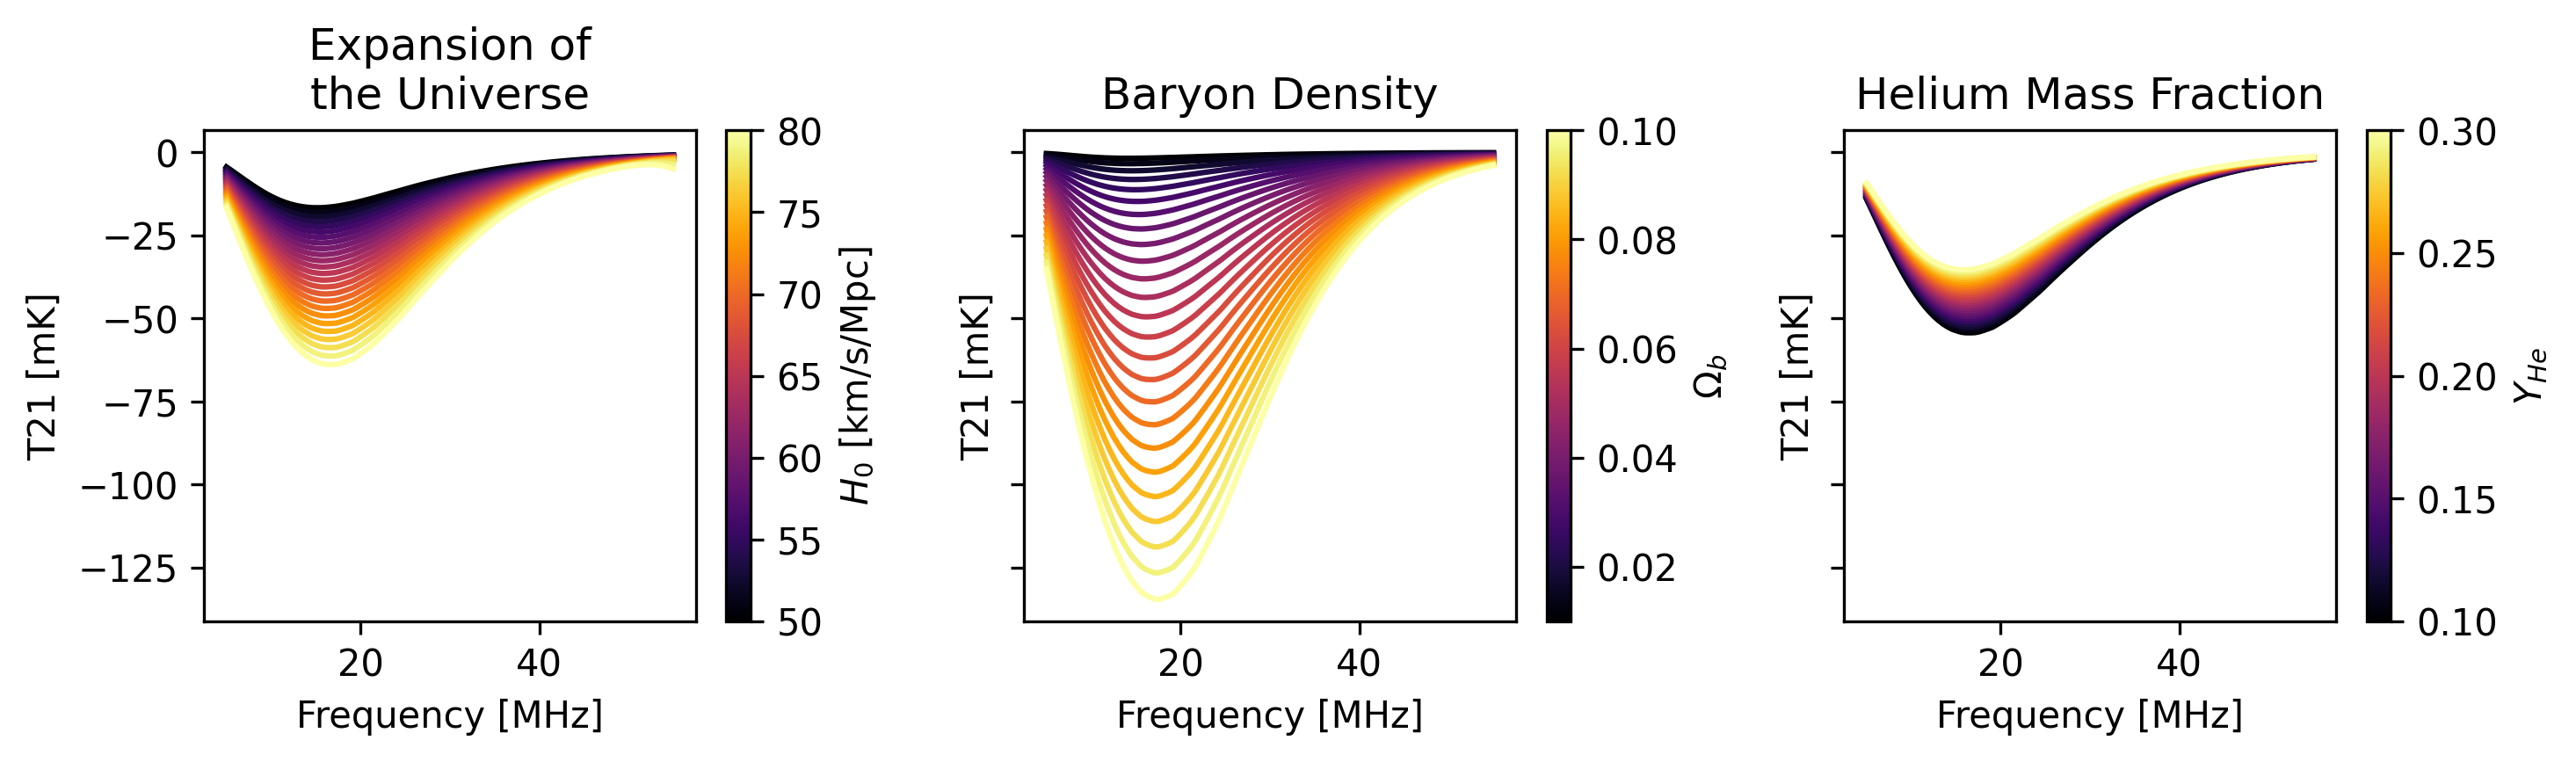
\includegraphics[width=0.99\linewidth]{figs/vary_cosmology.png}
    \vspace{0.5em}
    \centering
    {\footnotesize Using \texttt{hyprfine} code to exploe how the 21-cm signal varies around a fiducial Planck Cosmology. See \url{https://github.com/htjb/hyprfine}.}
\end{frame}

% How does the signal vary with cosmological parameters... 
\begin{frame}{$\Lambda$-CDM Cosmology}
    \centering
    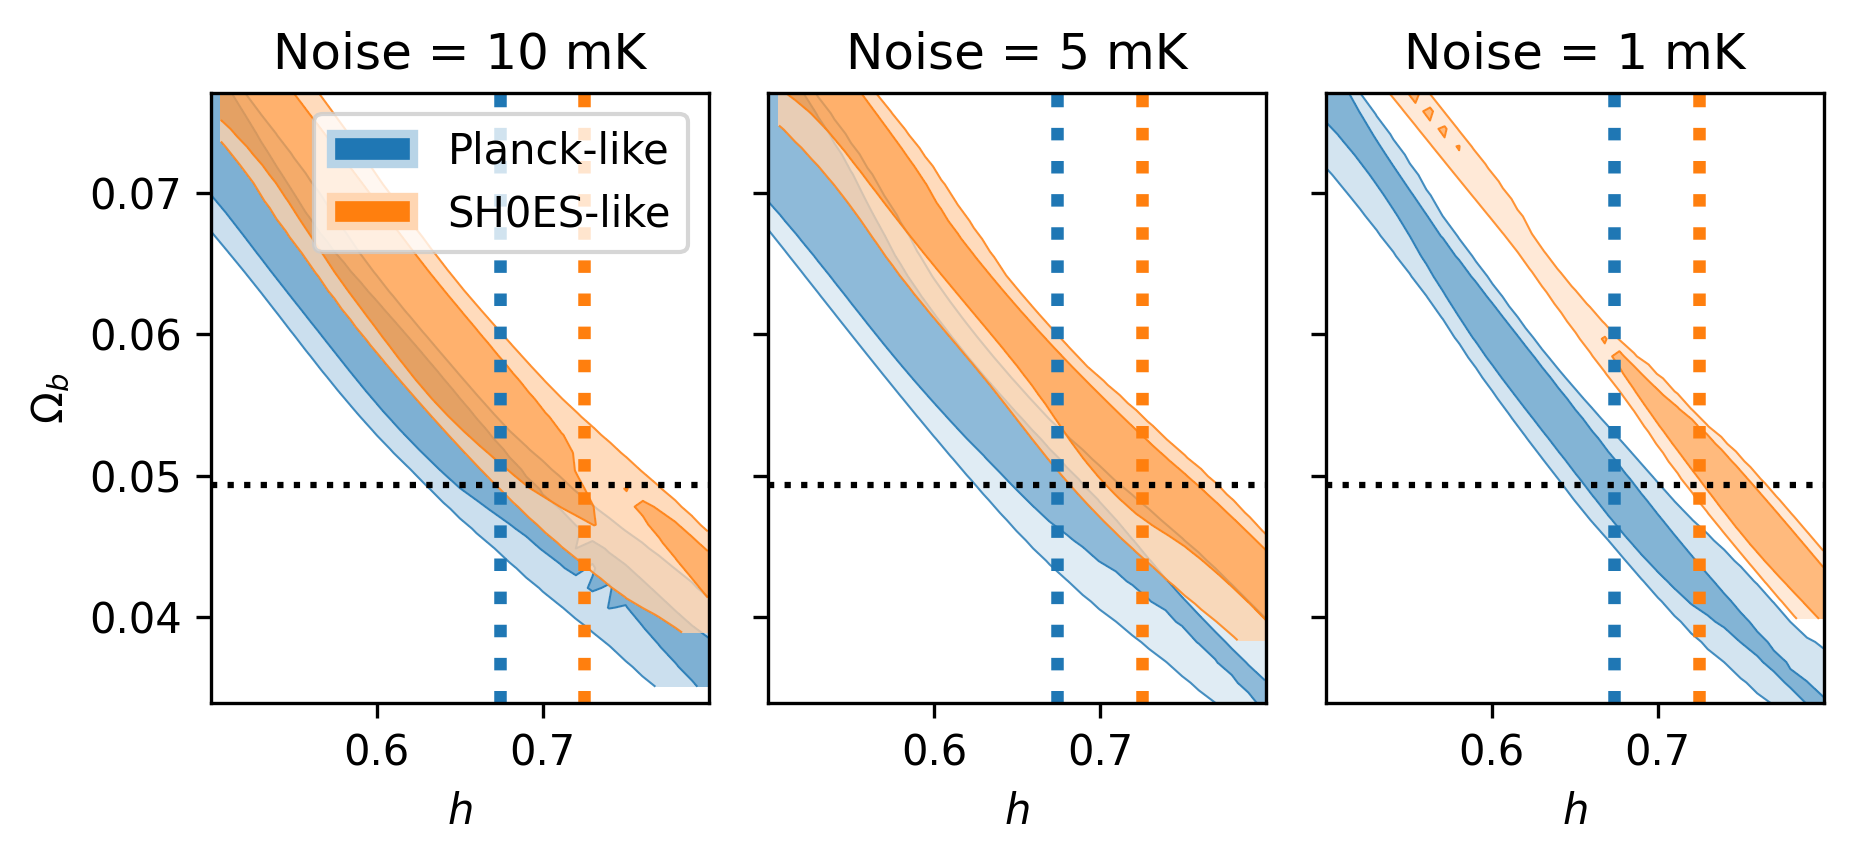
\includegraphics[width=0.8\linewidth]{figs/h_omegab_constraints_noise_comparison.png}
\end{frame}

%  Beyond lambda CDM
\begin{frame}{Beyond $\Lambda$-CDM}
    \begin{columns}[T]
        \begin{column}{0.30\textwidth}
            \centering
            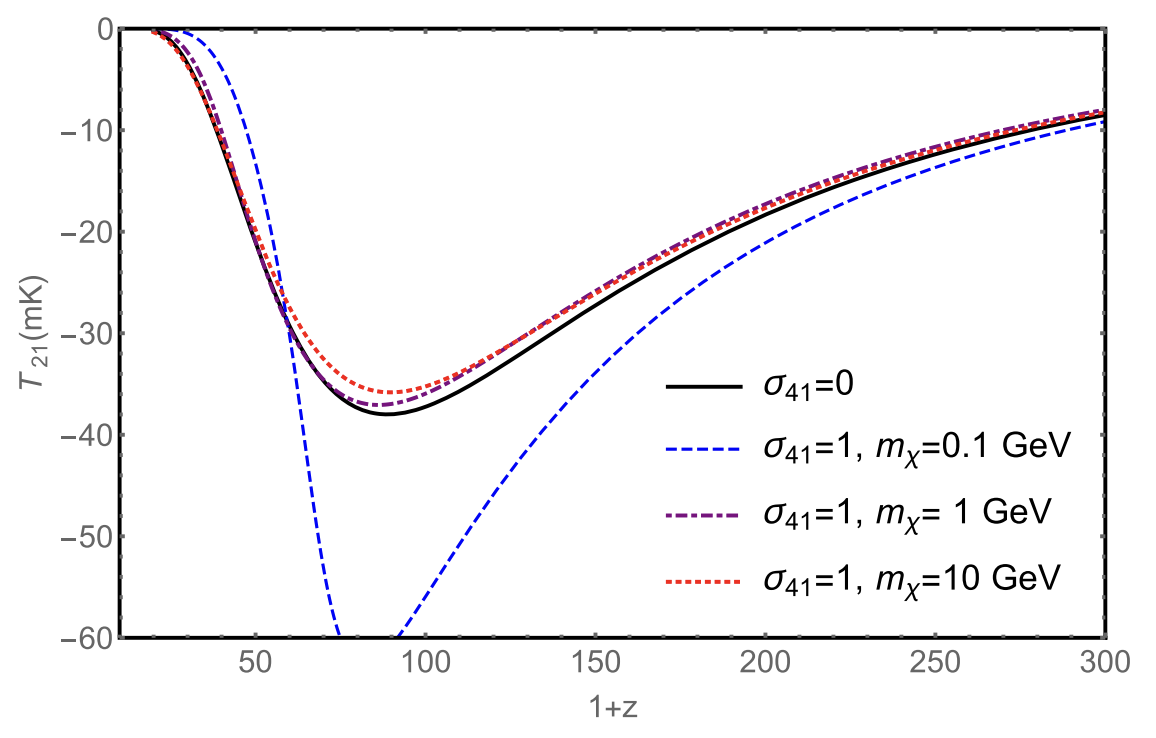
\includegraphics[width=\textwidth]{figs/Munoz-et-al.png}
            {\footnotesize Munoz et al. PRD 2015 \\ \begin{itemize} \item DM-Baryon Interactions \end{itemize}}
        \end{column}
        \begin{column}{0.30\textwidth}
            \centering
            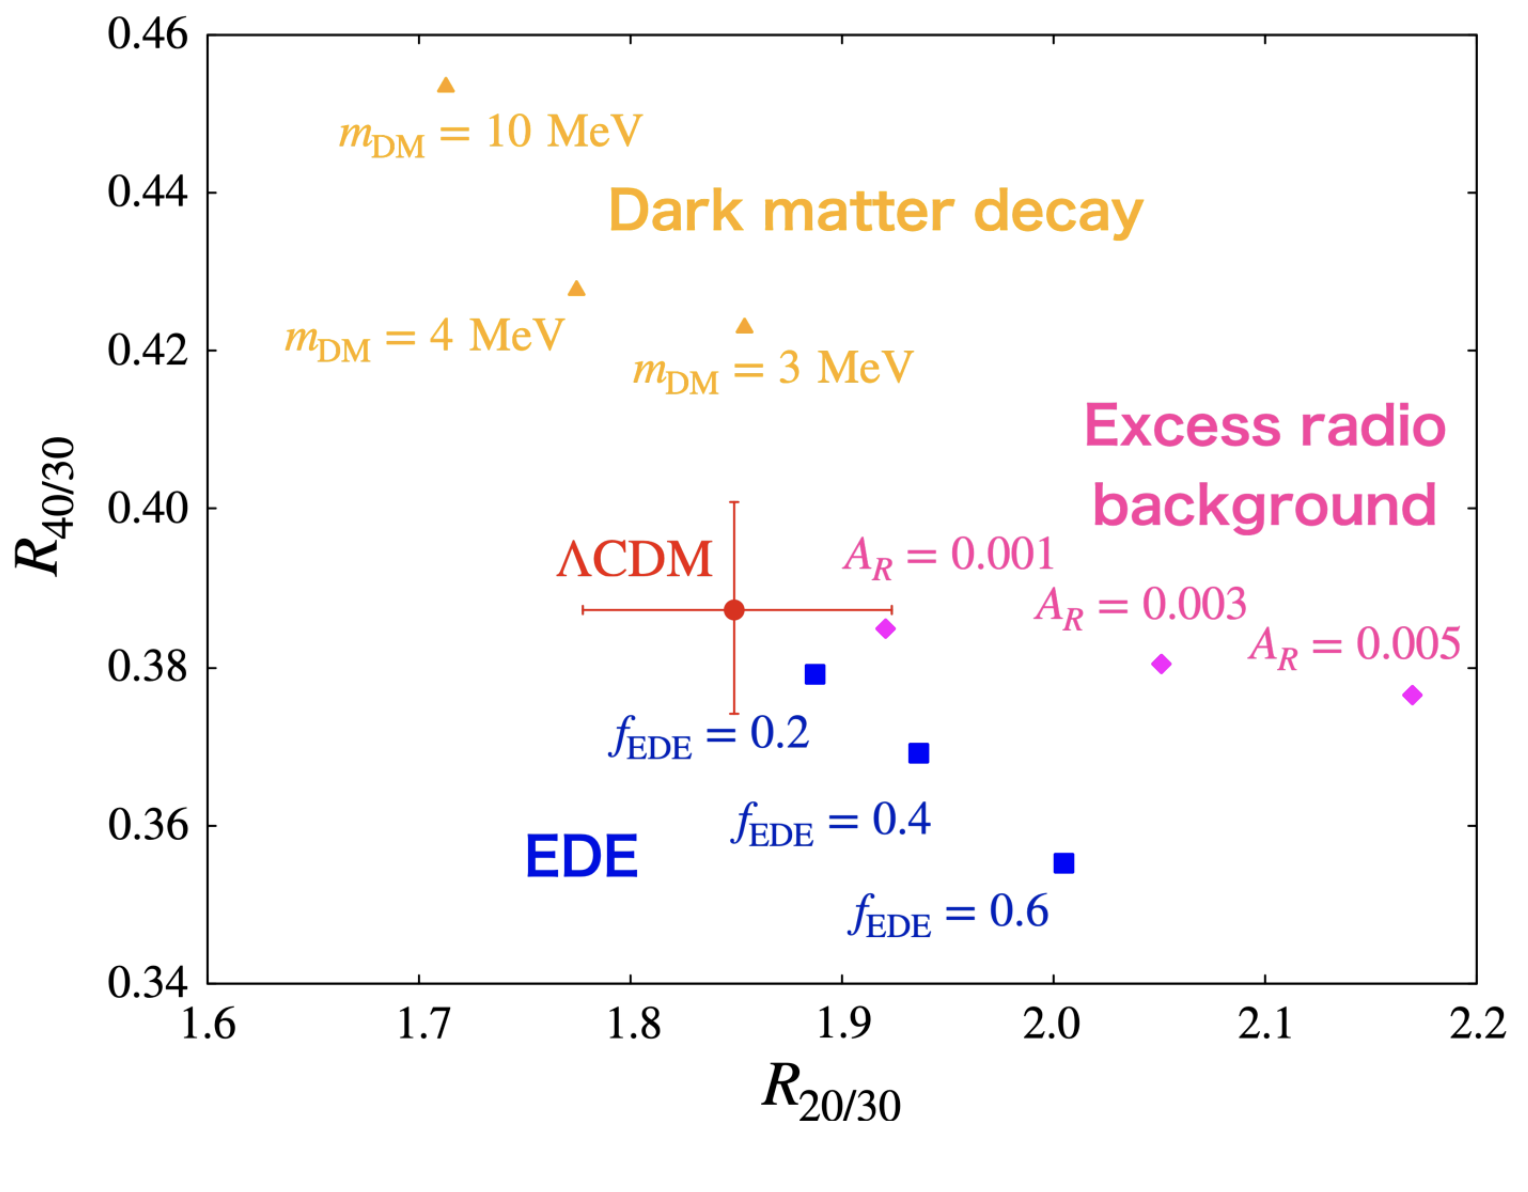
\includegraphics[width=\textwidth]{figs/Okamatsu-et-al.png}
            {\footnotesize Okamatsu et al. PRL 2024 \\ \begin{itemize} \item DM decay \item EDE \item Excess Radio Background \end{itemize}}
        \end{column}
        \begin{column}{0.35\textwidth}
            \centering
            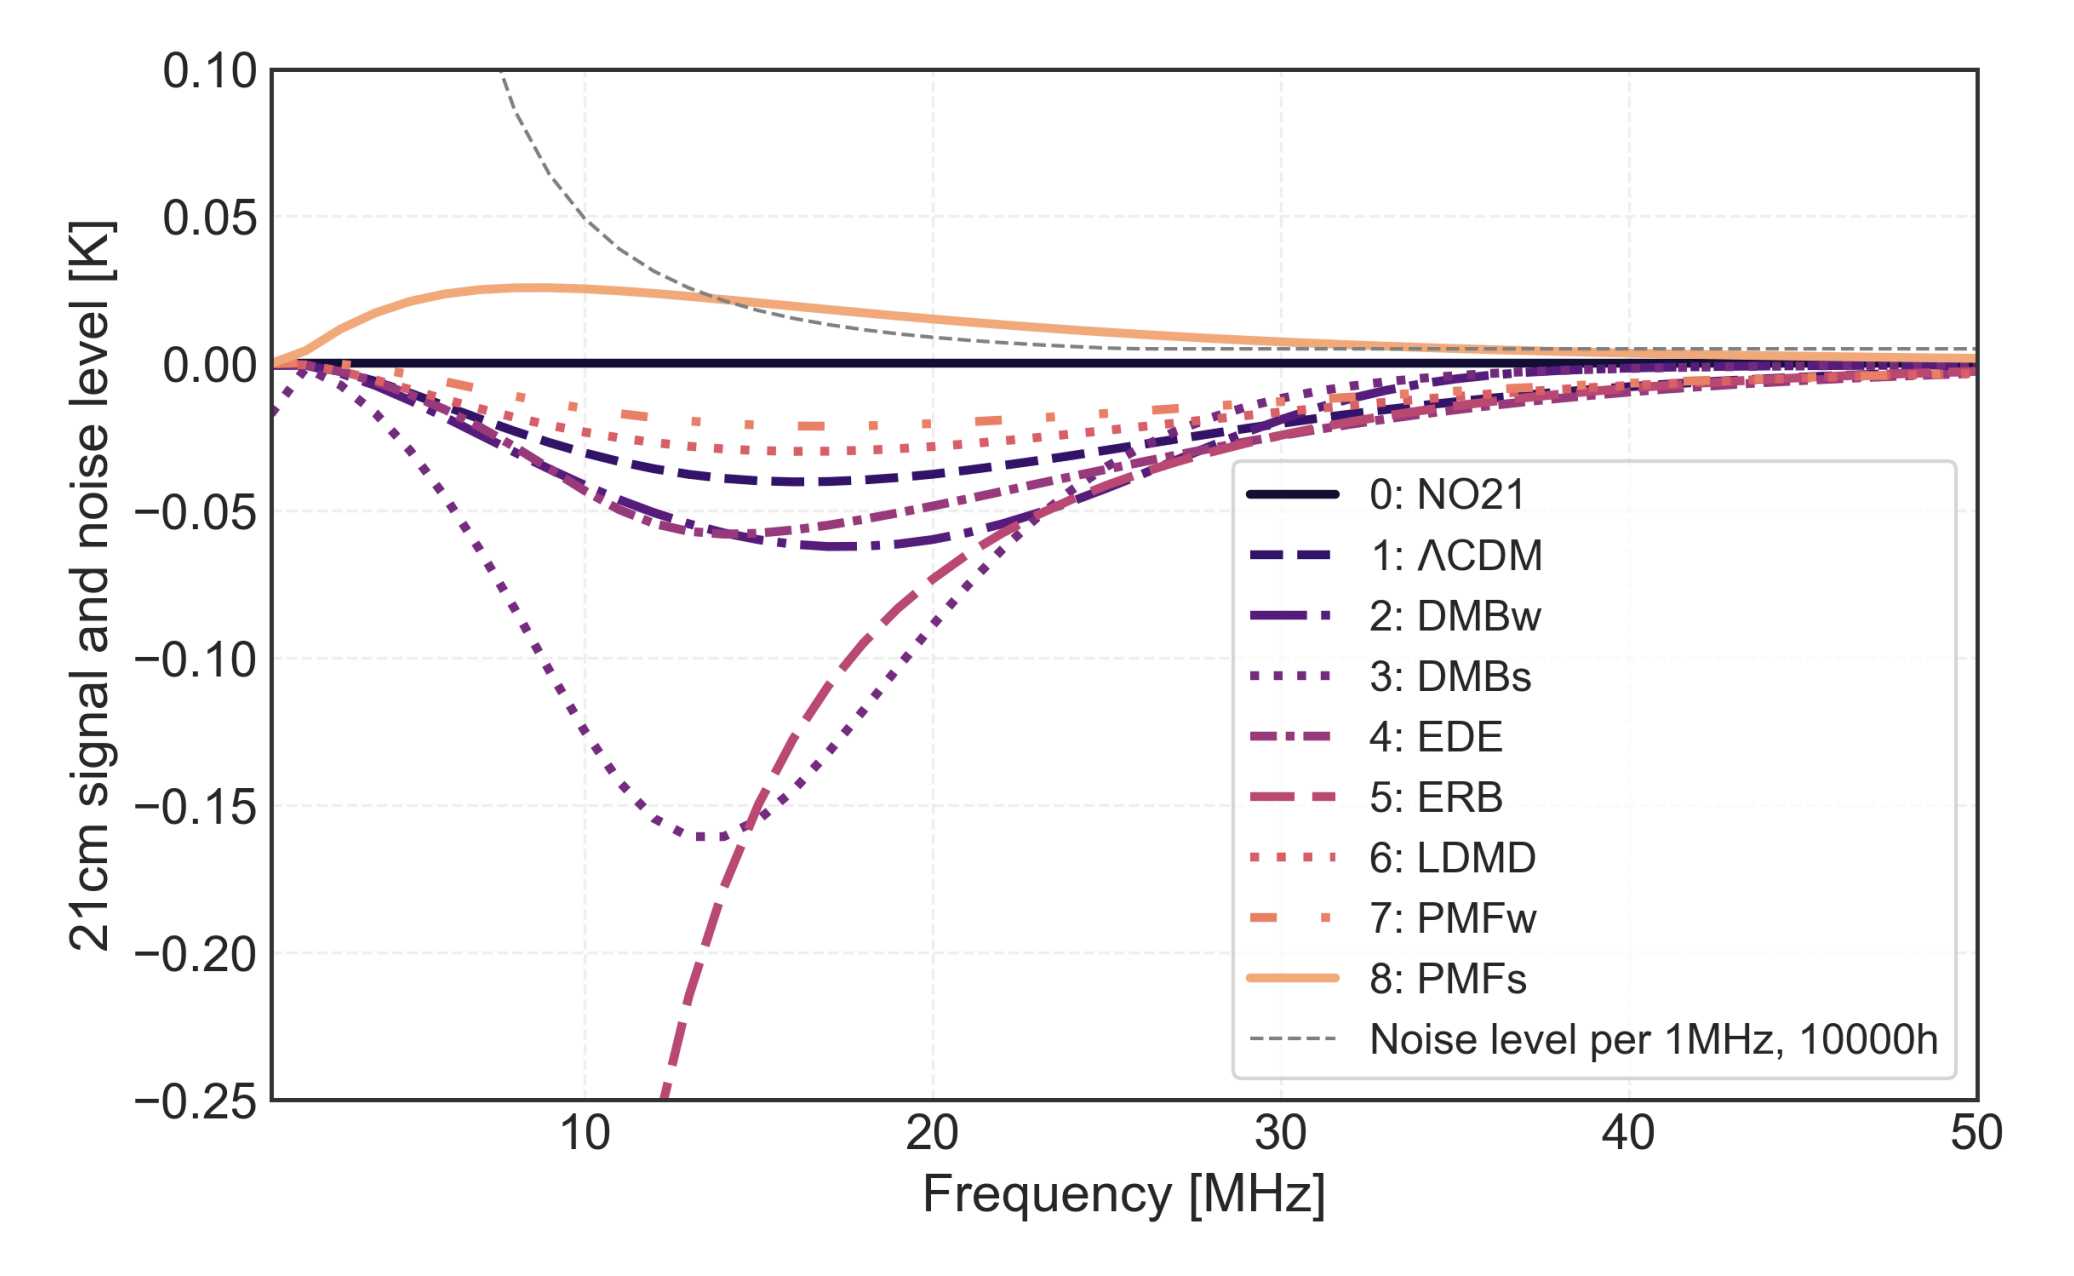
\includegraphics[width=\textwidth]{figs/Yoshiura-et-al.png}
            {\footnotesize Yoshiura et al. 2026 \begin{itemize} \item Primordial Magnetic Fields \end{itemize}}
        \end{column}
    \end{columns}
\end{frame}

\sectionframe{Lunar orbit, CosmoCube and the race back to the Moon}

% Why go to the moon
\begin{frame}{Why go to the moon?}
    \begin{columns}[T]
        \begin{column}{0.48\textwidth}
            \begin{itemize}
                \item Bullet pointing to the figure on the right
                \item Another bullet point
                \item And another one
                \item Sub-item example:
                      \begin{itemize}
                          \item Sub-point one
                          \item Sub-point two
                      \end{itemize}
            \end{itemize}
        \end{column}
        \hfill
        \begin{column}{0.48\textwidth}
            \centering
            \includegraphics[width=\textwidth]{example-image}  % replace with figure
            \\[0.3em]
            {\small Optional caption text}
        \end{column}
    \end{columns}
\end{frame}


% The race to the moon...
\begin{frame}{Radio Astronomy on the Moon?}
    \begin{columns}[T]
        \begin{column}{0.48\textwidth}
            \begin{itemize}
                \item Bullet pointing to the figure on the right
                \item Another bullet point
                \item And another one
                \item Sub-item example:
                      \begin{itemize}
                          \item Sub-point one
                          \item Sub-point two
                      \end{itemize}
            \end{itemize}
        \end{column}
        \hfill
        \begin{column}{0.48\textwidth}
            \centering
            \includegraphics[width=\textwidth]{example-image}  % replace with figure
            \\[0.3em]
            {\small Optional caption text}
        \end{column}
    \end{columns}
\end{frame}

% Cosmocube
\begin{frame}{CosmoCube}
    \begin{columns}[T]
        \begin{column}{0.48\textwidth}
            \begin{itemize}
                \item Bullet pointing to the figure on the right
                \item Another bullet point
                \item And another one
                \item Sub-item example:
                      \begin{itemize}
                          \item Sub-point one
                          \item Sub-point two
                      \end{itemize}
            \end{itemize}
        \end{column}
        \hfill
        \begin{column}{0.48\textwidth}
            \centering
            \includegraphics[width=\textwidth]{example-image}  % replace with figure
            \\[0.3em]
            {\small Optional caption text}
        \end{column}
    \end{columns}
\end{frame}



\sectionframe{Progress with CosmoCube}

% Platform
\begin{frame}{The Platform}
    \begin{columns}[T]
        \begin{column}{0.48\textwidth}
            \begin{itemize}
                \item Bullet pointing to the figure on the right
                \item Another bullet point
                \item And another one
                \item Sub-item example:
                      \begin{itemize}
                          \item Sub-point one
                          \item Sub-point two
                      \end{itemize}
            \end{itemize}
        \end{column}
        \hfill
        \begin{column}{0.48\textwidth}
            \centering
            \includegraphics[width=\textwidth]{example-image}  % replace with figure
            \\[0.3em]
            {\small Optional caption text}
        \end{column}
    \end{columns}
\end{frame}

% Payload
\begin{frame}{The Payload} 
    \centering
    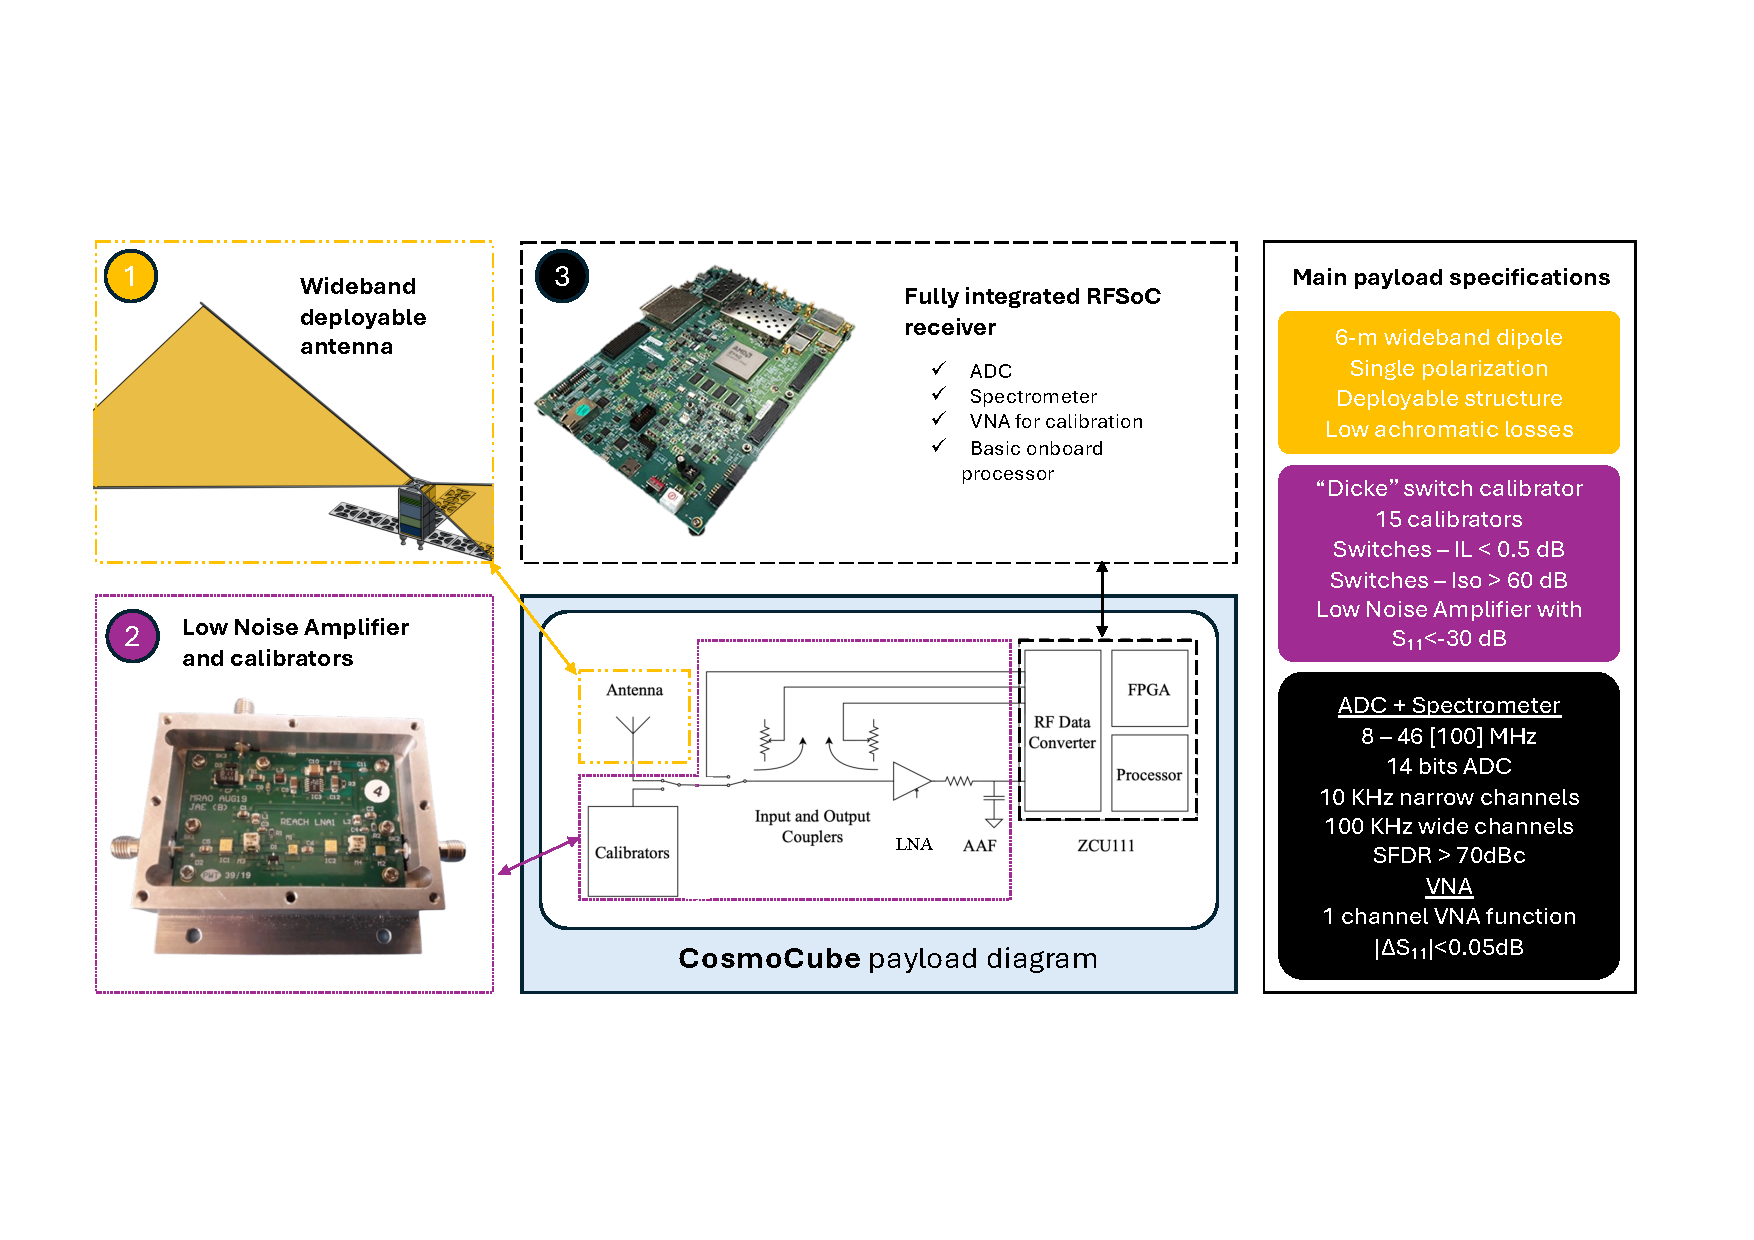
\includegraphics[width=\textwidth]{figs/CosmoCube_diagram.pdf}
\end{frame}

% Funding and status 
\begin{frame}{The Journey to Launch}
    \begin{columns}[T]
        \begin{column}{0.48\textwidth}
            \begin{itemize}
                \item Bullet pointing to the figure on the right
                \item Another bullet point
                \item And another one
                \item Sub-item example:
                      \begin{itemize}
                          \item Sub-point one
                          \item Sub-point two
                      \end{itemize}
            \end{itemize}
        \end{column}
        \hfill
        \begin{column}{0.48\textwidth}
            \centering
            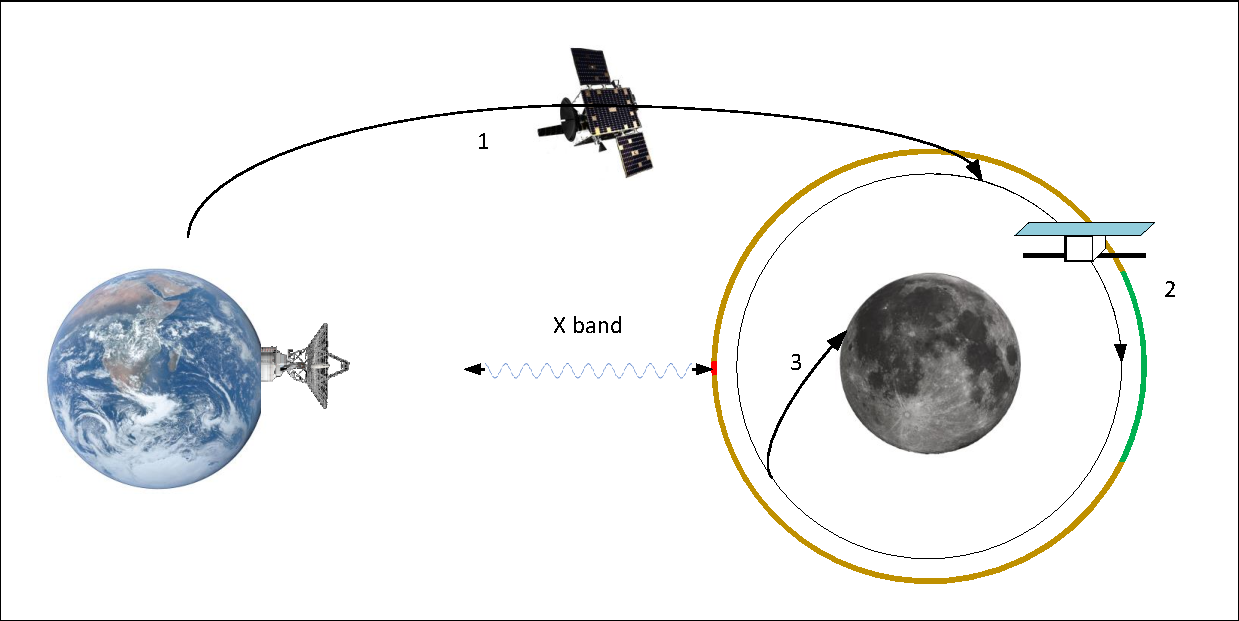
\includegraphics[width=\textwidth]{figs/cosmocube-lifecycle.pdf}  % replace with figure
            \\[0.3em]
            {\small Optional caption text}
        \end{column}
    \end{columns}
\end{frame}

% ── Highlighted text (uses accent colour) ────────────────────────────────────
\begin{frame}{Summary}
    \begin{itemize}
        \item Normal text looks like this
        \item \textcolor{accentblue}{Highlighted text in navy blue}
        \item Back to normal text
    \end{itemize}
\end{frame}

% ══════════════════════════════════════════════════════════════════════════════
\end{document}
